\documentclass[12pt]{article}

\usepackage[english]{babel}
\usepackage[utf8]{inputenc}
\usepackage[T1]{fontenc}
\usepackage{graphicx}
\usepackage{caption}
\usepackage{anysize}
\usepackage{amsmath}

\usepackage{hyperref}
\graphicspath{ {img/} }
\hypersetup{
	pdftitle = {IS - TP3}
	,pdfauthor = {João Ferreira \& João Silva\\ Departamento de Engenharia Informática\\ Universidade De Coimbra\\ \texttt{jpbat@student.dei.uc.pt | jfmsilva@student.dei.uc.pt}}
	,pdfborder = {0 0 0}
}

\title{Enterprise Application Integration \\ Practical Assignment 3}
\author{
		João Ferreira \& João Silva\\
		Departamento de Engenharia Informática\\
		Universidade de Coimbra\\
		\texttt{jpbat@student.dei.uc.pt | jfmsilva@student.dei.uc.pt}\\
		\texttt{2009113274 | 2008111448}
		}
\date{December 2013}

\begin{document}
\maketitle
\clearpage

\tableofcontents

\setlength{\parindent}{1cm}
\setlength{\parskip}{0.3cm}

\clearpage
\section{Introduction}
\indent \indent In this practical assignment it was requested that we reused the first one (just the crawler) to generate a xml file. Only one adjustment had to be made, so that the rate of the movie was also fetched.

We also needed to send emails to subscription clients and post some tweets. The twitter account used can be found in \href{https://twitter.com/IMDbCrawler}{@IMDbCrawler}.

We'll now briefly explain some decisions that were taken and how we solved some issues that appeard along the way.

\section{Data Model}
\indent \indent As it is obvious not all the information that is obtainded by the crawler is needed, so we decided to change our database desing.

\begin{figure}[h!]
	\centering
	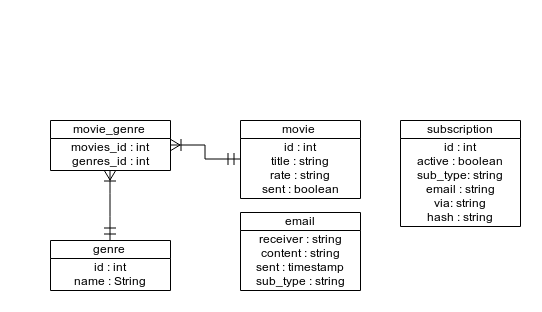
\includegraphics[width=\textwidth]{er.png}
	\caption{ER Model.}
\end{figure}
\clearpage

\section{Flows}
\indent \indent We created three separated flows files, being the first to movie subscription, the second to movie management and the last retreives the stats.

\subsection{Movie Subscription}
\indent In this flow we added the actions to subscribe/unsubscribe to the service. Either by SOAP or via Web, the first step is always to save the data into Session Variables so that we can develop a more dynamic application.

\begin{figure}[h!]
	\centering
	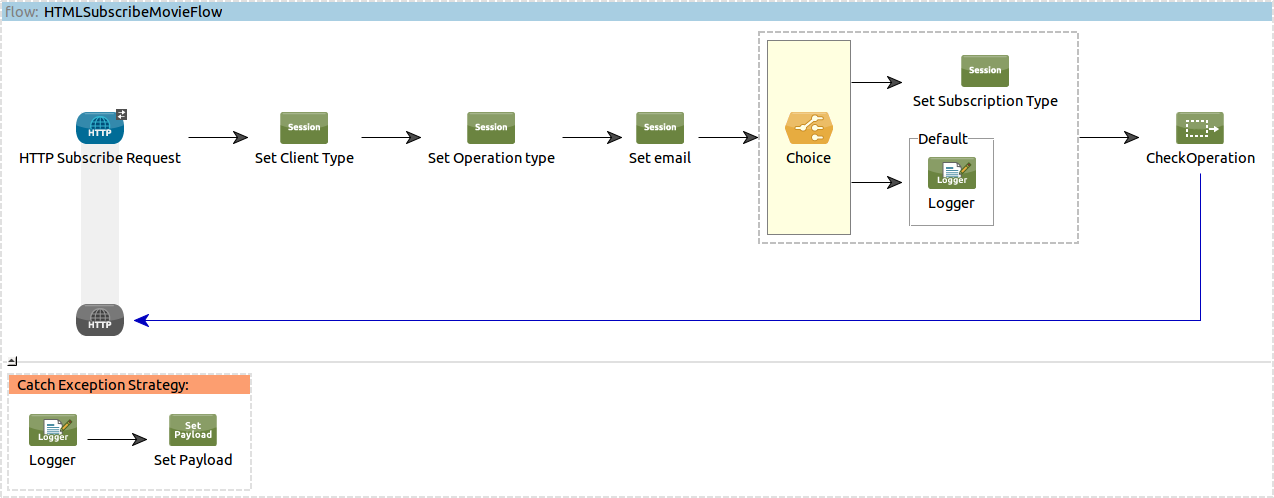
\includegraphics[width=\textwidth]{HTMLSubscribeMovieFlow.png}
	\caption{Data extraction on WEB}
\end{figure}
\begin{figure}[h!]
	\centering
	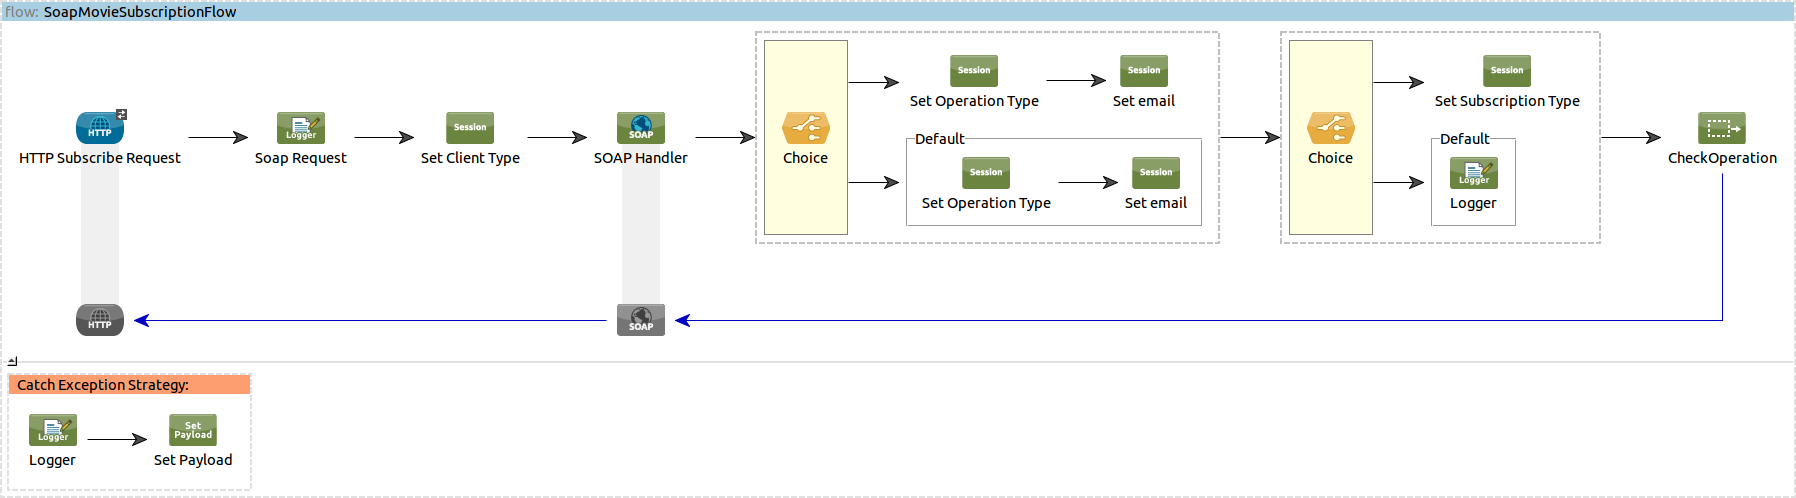
\includegraphics[width=\textwidth]{SoapMovieSubscriptionFlow.png}
	\caption{Data extraction on SOAP}
\end{figure}
\clearpage

After this the application chooses if it should perform a subscription or an unsubscription.

\begin{figure}[h!]
	\centering
	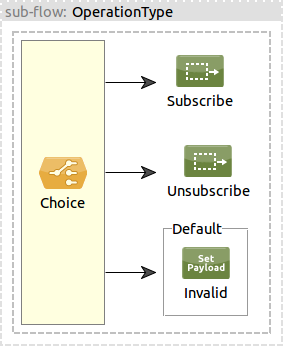
\includegraphics[width=5cm]{OperationType.png}
	\caption{Choosing the type of operation}
\end{figure}

Deppending on the operation the application will perform one of the two folowing flows.

\begin{figure}[h!]
	\centering
	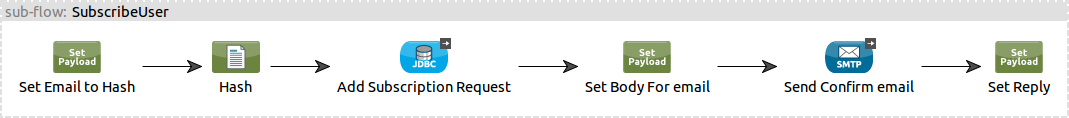
\includegraphics[width=\textwidth]{SubscribeUser.png}
	\caption{Subscribing a user}
\end{figure}

On the first we start by calculating an hash that is going to be used to activate the subscription. after that we insert all that information into the database. Finnaly we send an email with the link to the activation of said subscription.

\begin{figure}[h!]
	\centering
	
\includegraphics[width=\textwidth]{unSubscribeUser.png}
	\caption{Unsubscribing a user}
\end{figure}

On the second we delete from the database the subscription which contained the providaded email. After that we send an email confirming the deactivation of the subscription.
\clearpage
By last we have a flow that changes the status of the subscription when the user follows the link provided in the email that was sent.

\begin{figure}[h!]
	\centering
	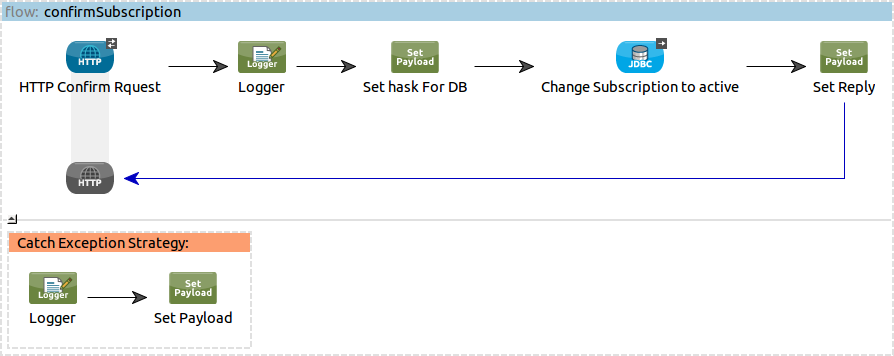
\includegraphics[width=\textwidth]{confirmSubscription.png}
	\caption{Confirming Subscription}
\end{figure}
\clearpage

\subsection{Movie Manage}
\indent \indent In this flow we have three main flows.

The first two are to add movies either via putting a file in the trigger folder, or by using the SOAP client wich is integrated in the crawler from the first project.

\begin{figure}[h!]
	\centering
	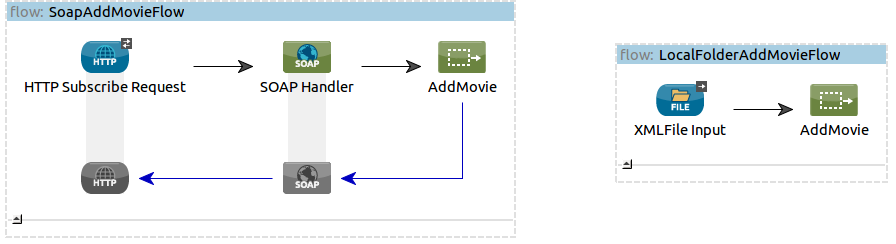
\includegraphics[width=\textwidth]{addFlows.png}
	\caption{Both flows to add movies}
\end{figure}

After this we jump into a subflow that is responsible for storing the movie into the database, sending tweets and also sending the digest email as well as storing the information about the sent email into the database so that we can produce stats.
The conversion of the XML string into object is done by using JAXB generated classes from the first project.

\begin{figure}[h!]
	\centering
	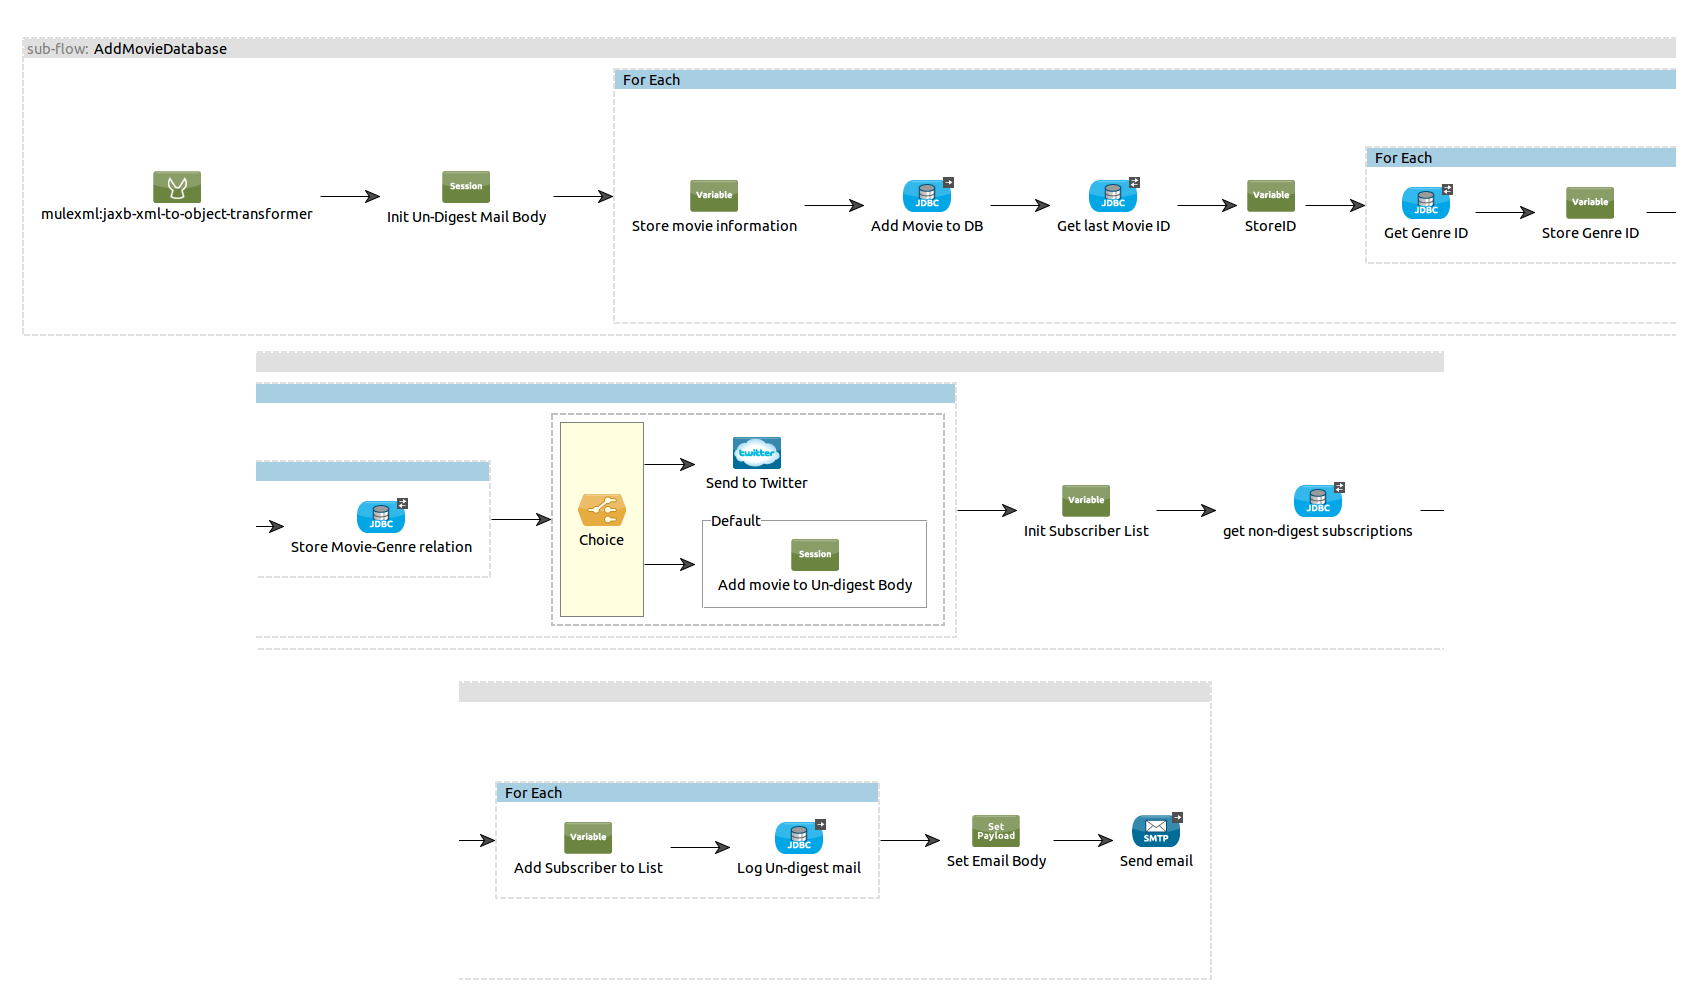
\includegraphics[width=\textwidth]{AddMovieDatabase.png}
	\caption{Add movie to database}
\end{figure}
\clearpage

The third flow is the one that is responsable by sending the digest emails, based on a quartz event dispatcher.

\begin{figure}[h!]
	\centering
	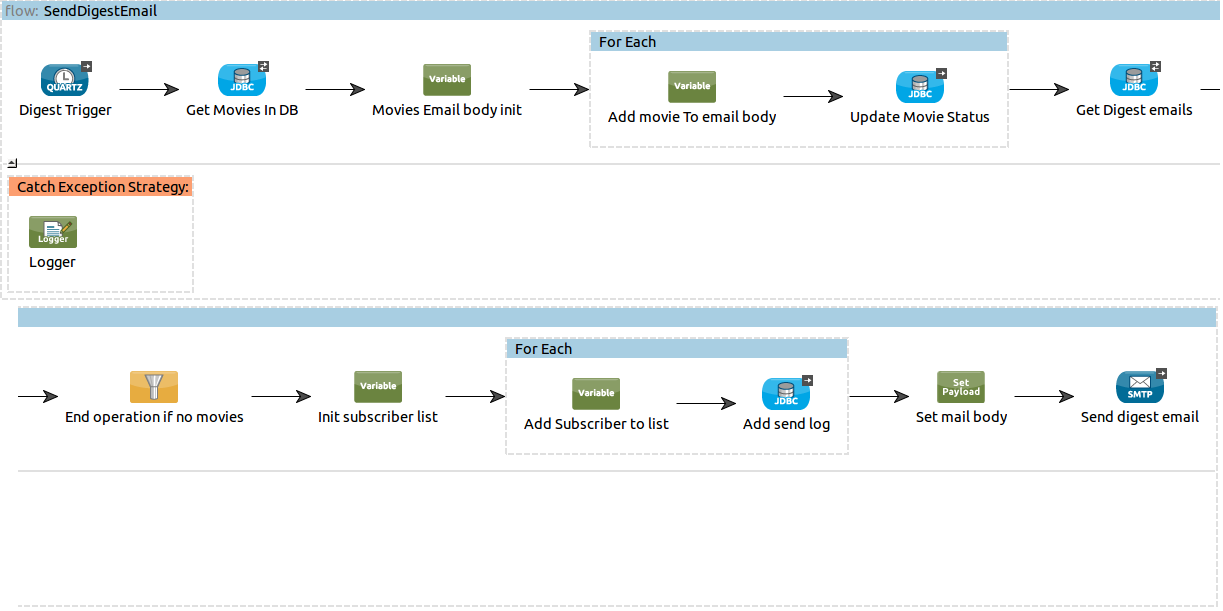
\includegraphics[width=\textwidth]{SendDigestEmail.png}
	\caption{Send digest emails}
\end{figure}
\clearpage

\subsection{Movie Stats}
\indent \indent This is by far the simplest flow, once all it does is queries to the database to retreive the information based on the selected option.

\begin{figure}[h!]
	\centering
	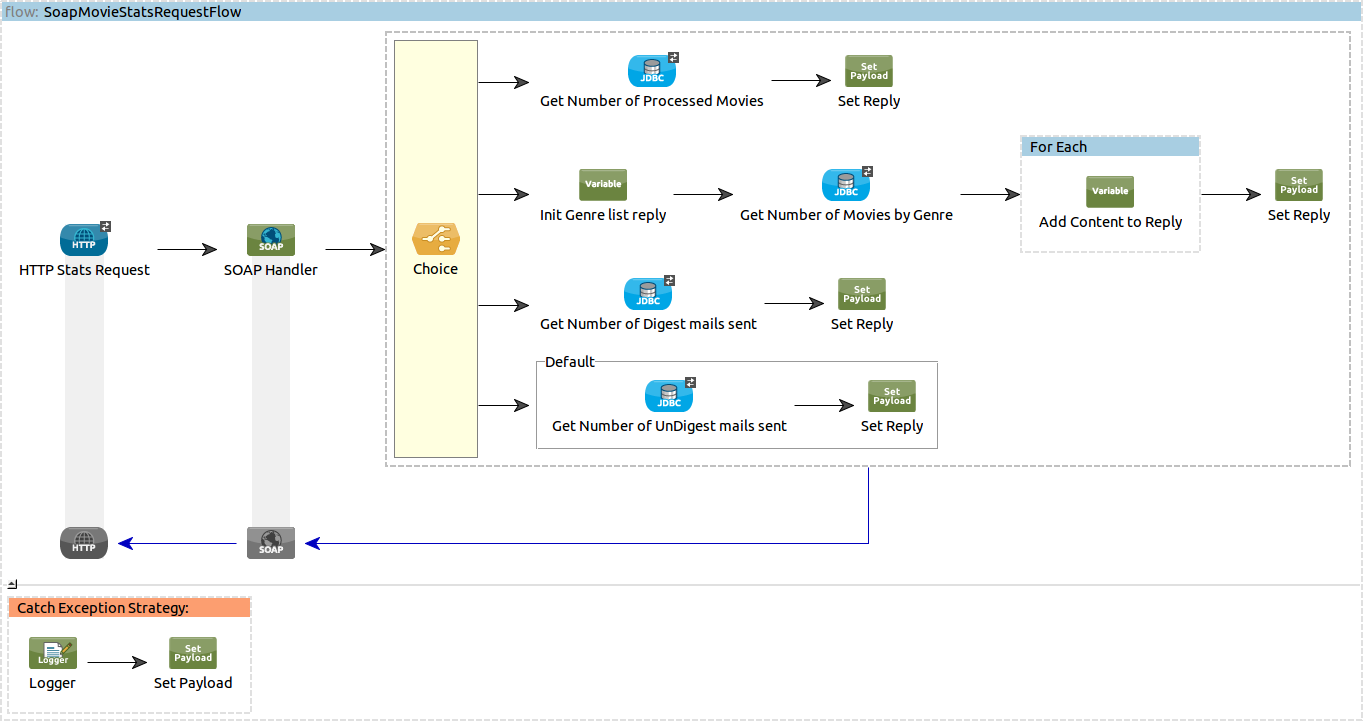
\includegraphics[width=\textwidth]{SoapMovieStatsRequestFlow.png}
	\caption{Stats Producer}
\end{figure}
\clearpage

\section{Division of Work}
\indent \indent The work was, in what appeard to us and as far as possible, equally divided.

Unfortunately we were unable to make a clear separation of the work. This happened because we couldn't develop at the same time, once the Mule Studio kept giving build issues. We even tried to add to our git repository the .gitignore that they recomended, which turned out to be a lost of time.

Also if we divided the project too much, one of us could easly loose track of the development state.

Ence this was the best division we could make.

\begin{description}
	\item [João Ferreira] Mule Flows, Database modeling. (50h)
	\item [João Silva] Mule Flows, SOAP clients. (50h)
\end{description}
\clearpage

\section{Conclusion}
\indent \indent With this project we learned how to use a SOAP client/server. 

Besides that we dont think that Mule Studio wasn't a good tool to use, once we crossed some bugs on it. For instance the returning value on an insert query is not supported, therefore obligating us to do yet another query, ence overloading the system. We also had some Twitter issues, to which the solution was remove the connector and add it again, we even tried to make the diff of the xml after that step and it was equal.

Maybe in the future the Mule Studio will be a good solution, for now we think its mediocre, once there are some bugs as it was refered and there could be more and better doccumentation.

Although all of this  we consider that the execution of this assignment was a success, for wich the both of us learned some important aspects of the importance of using tools to integrate severall services.
\clearpage
\end{document}